\section{Conclusion}
\label{sec:conclusion}

This laboratory provided us the opportunity to understand how the envelope detector and voltage regulator circuits work and also, how to improve their efficieny. We're also able to analyse carefully the working principle of an AC/DC converter. \par
In order to analyse the circuit theoreticaly \textit{Ocatve} was used as well as all the Kirchoff's equations and diode models that support this analysis. 
The simulation was done using \textit{Ngspice}. \par
Finally, we are going to compare the results from simulation and theoretical analysis side by side: \par
%compararações

\begin{center}
  \begin{tabular}{ | c | c | }
    \hline    
    {\bf Name} & {\bf Value} \\ \hline
    Resistor Cost & 3.315000e+01 \\ \hline 
Capacitor Cost & 2.600000e+01 \\ \hline 
Diode Cost & 2.300000e+00 \\ \hline 
Total Cost & 6.145000e+01 \\ \hline 
Merit & 2.591430e-01 \\ 

    \hline
  \end{tabular}
  \captionof{figure}{Merit Figure Table}
\end{center}

\begin{figure}[H]
    \minipage{0.45\textwidth}
      \includegraphics[width=\linewidth]{../mat/outputdc.pdf}
      \caption{Theoretical Output Voltage Level}
    \endminipage\hfill
    \minipage{0.45\textwidth}
      \includegraphics[width=\linewidth]{../sim/transient1.pdf}
      \caption{Simulation Output Voltage Level}
    \endminipage\hfill
\end{figure}

\begin{center}
  \begin{tabular}{ | c | c | }
    \hline    
    {\bf Name} & {\bf Value [V]} \\ \hline
    \input{../mat/ripple_octave}
    \hline
  \end{tabular}
  \captionof{figure}{Theoretical Ripple}
\end{center}

\begin{center}
  \begin{tabular}{ | c | c | }
    \hline    
    {\bf Name} & {\bf Value [V]} \\ \hline
    \input{ripple_tab}
  \end{tabular}
  \captionof{figure}{Simulation Ripple}
\end{center}

\begin{figure}[H]
    \minipage{0.45\textwidth}
      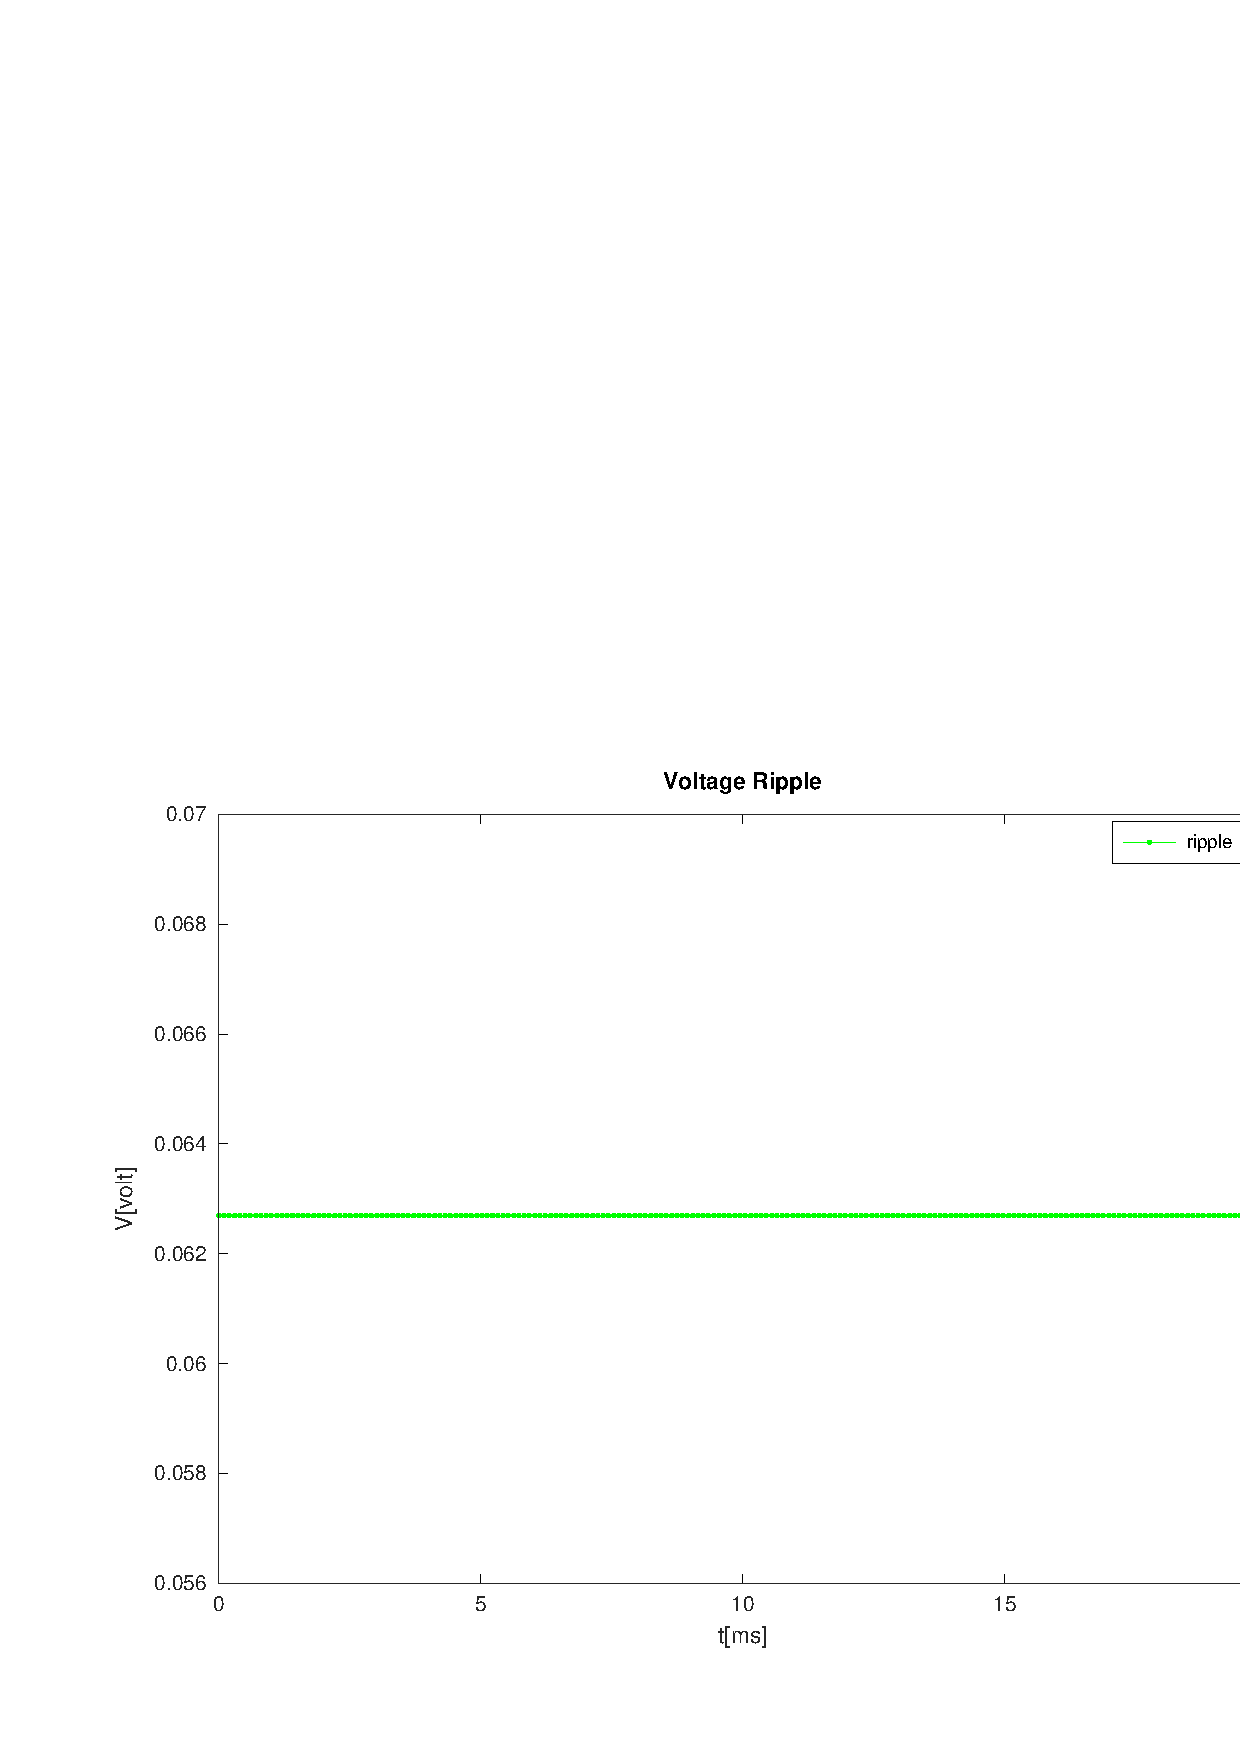
\includegraphics[width=\linewidth]{../mat/ripple.pdf}
      \caption{Theoretical Ripple}
    \endminipage\hfill
    \minipage{0.60\textwidth}
      \centering
      \begin{tabular}{ | c | c | }
      \hline    
      {\bf Ripple} & {\bf Value [V]} \\ \hline
      \input{ripple_tab}
      \end{tabular}
      \caption{Simulation Ripple}
    \endminipage\hfill
\end{figure}

\begin{figure}[H]
    \minipage{0.45\textwidth}
      \includegraphics[width=\linewidth]{../mat/envelope.pdf}
      \caption{Theoretical Envelope Detector Voltage Level}
    \endminipage\hfill
    \minipage{0.45\textwidth}
      \includegraphics[width=\linewidth]{../sim/transient2.pdf}
      \caption{Simulation Envelope Detector Voltage Level}
    \endminipage\hfill
\end{figure}

\begin{figure}[H]
    \minipage{0.45\textwidth}
      \includegraphics[width=\linewidth]{../mat/outputdc.pdf}
      \caption{Theoretical Voltage Regulator Voltage Level}
    \endminipage\hfill
    \minipage{0.45\textwidth}
      \includegraphics[width=\linewidth]{../sim/transient3.pdf}
      \caption{Simulation Voltage Regulator Voltage Level}
    \endminipage\hfill
\end{figure}

\begin{figure}[H]
    \minipage{0.45\textwidth}
      \includegraphics[width=\linewidth]{../mat/v012.pdf}
      \caption{Theoretical $v_0-12$ Voltage Level}
    \endminipage\hfill
    \minipage{0.45\textwidth}
      \includegraphics[width=\linewidth]{../sim/transient5.pdf}
      \caption{Simulation $v_0-12$ Voltage Level}
    \endminipage\hfill
\end{figure}